\documentclass[10pt, notumble, letterpaper]{leaflet}
\usepackage[spanish,mexico]{babel}
\usepackage[utf8]{inputenc}
\usepackage{fancyhdr} 
\pagestyle{fancy}
\fancyhf{}
\cfoot{\thepage}	
\usepackage[usernames]{xcolor}
\usepackage{float} 
\usepackage{multirow}

\usepackage{amsmath}		
\usepackage{amssymb}		
\usepackage{amsfonts}
\usepackage{latexsym}
\usepackage{graphicx}
\usepackage{cite}

\title{\textbf{Trípticos con \LaTeX}}
\author{Jesús Esteban Sánchez Alcántara\\chuyunam93@gmail.com}

%Marcas que dividen al triptico
\CutLine*{1}% linea punteada sin tijeras
\CutLine*{3}% linea punteada sin tijeras
\CutLine{4}% linea punteada sin tijeras
\CutLine{6}% linea punteada con tijeras

\begin{document}
\renewcommand{\contentsname}{Temas en general}
\pagecolor{yellow}
\maketitle
\tableofcontents
\listoffigures
\listoftables


\newpage
\pagecolor{white}%Aqui cambia nuevamente de color
\section{Trípticos usando la clase leaflet}
\begin{enumerate}
	\item Los trípticos se pueden realizar utilizando la clase beamer o la clase
	leaflet, esta última es una clase especializada para este tipo de documentos.
	\item Para este tríptico se uso la clase leaflet.
	\item En el caso de leaflet la segunda página aparece al revés para imprimir directamente en una impresora 	que imprima por ambos lados de la página. Sin embargo, si no se quiere que la segunda página aparezca de 		esta forma se debe colocar la opción \textbf{notumble}.
	\item Usar leaflet tiene la ventaja de que las seis páginas del tríptico se acomodan automáticamente en el 	código.
	\item Simplemente se escribe de manera contínua utilizando título, secciones, subsecciones, etc.
	\item En el momento que se acabe una página se continúa automáticamente en la página siguiente y si se 			quiere pasar de página de forma manual se puede utilizar el comando \verb@\newpage@.
	\item Con la clase leaflet podemos hacer diferencia entre las páginas, para que a la hora de armar el 			tríptico se puedan hacer los dobleces sin tener que estar haciendo mediciones. Por ejemplo,para trazar las 	líneas punteadas que separan las páginas pequeñas usamos el comando	\verb@\CutLine*{1}@ para hacer una 			línea punteada sin tijeras o \verb@\CutLine{6}@ para una línea punteada con tijeras.
\end{enumerate}
\textbf{Nota:estas instrucciones van en el preámbulo de nuestro documento}

\section{Otra sección}
También puede haber minisecciones o minicapítulos en el tríptico dependiendo de como lo queramos ver.Este es un ejemplo.

\newpage
\section{Expresiones matemáticas en un tríptico}
En resumen se pueden poner todos los símbolos usados en los otros tipos de documentos vistos a lo largo del curso. Por ejemplo, escribimos en \LaTeX{}:\\

\verb@$\sqrt[3]{25}$@ para que nos de $\sqrt[3]{25}$\\

\verb@$\frac{3}{7}$@ para que nos de $\frac{3}{7}$\\

\verb@$y^{2x^2}$@ para que nos de $y^{2x^2}$\\
\begin{verbatim}
\begin{pmatrix}
	1 & 2 \\
	3 & 4
\end{pmatrix}
\] 
\end{verbatim}

para que nos de
\[
\begin{pmatrix}
	1 & 2 \\
	3 & 4
\end{pmatrix}
\]\\

\verb@$\displaystyle \lim_{x\to 0} f(x)$@ para que nos de $\displaystyle \lim_{x\to 0} f(x)$

\verb@$a \leq b$@ para que nos de $a \leq b$\\

\verb@$a \geq b$@ para que nos de $a \geq b$\\

\verb@$a \in B$@ para que nos de $a \in B$\\

\newpage
\section{Imágenes en el tríptico}
Al igual que en los otros tipos de documentos,las figuras se pueden poner mediante las siguientes instrucciones: 
\begin{verbatim}
\begin{figure}[h!]
\centering
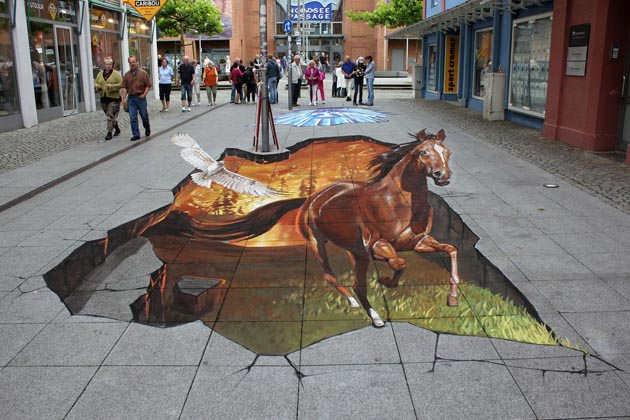
\includegraphics[scale=0.3]{caballo}
\caption{Caballo 3D} %Figura1
\end{figure}
\end{verbatim}

\begin{figure}[h!]
\centering
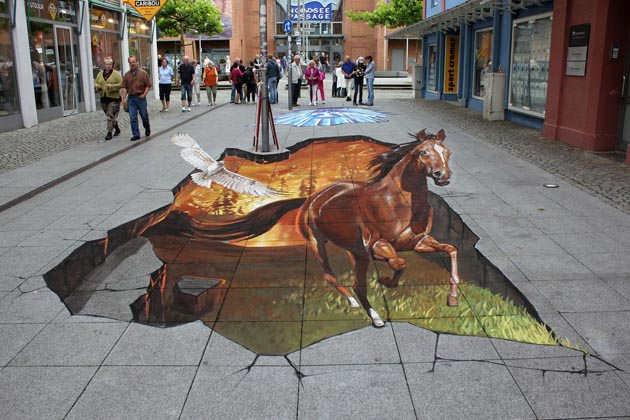
\includegraphics[scale=0.3]{caballo}
\caption{Caballo 3D}
\end{figure}

\begin{figure}[h!]
\centering

\includegraphics[angle=60,scale=0.3]{balondeMexico}
\caption{Balón de México rotado 60}
\end{figure}


\newpage
\section{Tablas en el tríptico}

Al igual que en los reportes, libros, artículos o presentaciones, con la clase leaflet en los trípticos podemos crear tablas con el entorno \verb@tabular@ puede ser incluido dentro del entorno \verb@table@ para agregar algunas características a la tabla.
\begin{table}[h!]
\centering
\begin{tabular}{|c|c|c|} \hline
$p$ & $q$ & $p \rightarrow q$\\\hline
0 & 0 & 1 \\
0 & 1 & 1 \\
1 & 0 & 0 \\
1 & 1 & 1 \\\hline
\end{tabular}
\caption{Tabla de verdad del implica}
\end{table}

Con el comando \verb@\hline@ se indica que se deben colocar líneas horizontales a la tabla.\\
Con el comando \verb@\cline{i-j}@ se indica una línea de la columna i a la j.

\begin{table}[h!]
\centering
\begin{tabular}{|c|c|} \hline
\multirow{2}{*}{Raíz} & \multirow{2}{*}{$\sqrt[3]{56}$} \\
& \\ \hline
\multirow{2}{*}{Potencia} & \multirow{2}{*}{$x^3$} \\
& \\ \hline
\multirow{2}{*}{Fracción} & \multirow{2}{*}{$\frac{1}{3}$} \\
& \\ \hline
\multirow{2}{*}{Límite} & \multirow{2}{*}{$\displaystyle \lim_{x\to 0} f(x)$} \\
& \\ \hline
\multirow{2}{*}{Integral} & \multirow{2}{*}{$\int \! g(x) \, \mathrm{d}x $} \\
& \\ \hline
\end{tabular}
\caption{Expresiones matemáticas}
\end{table}

\textbf{Nota:las tablas que se pongan deben de ser lo suficientemente chicas para que quepan en el tríptico ya que de lo contrario se pueden llegar a salir y a la hora de reajustarla se puede ver la información muy pequeña.}

\newpage
\section{Otras cosas}
En los trípticos, las secciones en las que esta dividido pueden ir de diferente color. Por ejemplo, la portada de esta tríptico esta de color amarillo  mientras que las demás secciones estan en blanco.\\

También se puede apreciar que pueden tener su pie de página. Se fueron enumerando en este orden ya que así es como se formará el tríptico.
Si se pusiera de nuevo \verb@\newpage@ y se pusiera otra sección o contenido ya no se mostrarían en el tríptico puesto que ya no habría espacio para poner más cosas.\\

{\color {red}{Podemos cambiar de color las letras o}} \underline{ponerlas subrayadas}.\\

También se pueden poner las palabras, imagenes, expresiones o cualquier cosa con recuadros, por ejemplo:\\

\verb@\fbox{Hola que hace}@ nos da \fbox{Hola que hace}\footnote{Este texto puede ir de color y en itálicas también}\\

Para más información sobre alguna otra cosa que se puede hacer con los trípticos vea \cite[cap.13]{LATEX 2014}

\begin{thebibliography}{99}
\bibitem{LATEX 2014} Borbón A.,Alexánder; Edición de textos científicos, LATEX 2014; Revista digital Matemática, Educación e Internet; 2014.
\end{thebibliography}

\end{document}
